% ch06_algorithm.tex
% Chapter 6: תכנון תנועה אדפטיבי לניווט בסביבות משתנות באמצעות למידת חיזוק מבוזרת
% Compiler: XeLaTeX

\selectlanguage{hebrew}

\section{תכנון תנועה אדפטיבי לניווט בסביבות משתנות באמצעות למידת חיזוק מבוזרת}
\label{sec:ch06_rl_planning}

\subsection{מרחב מצב ופעולה לרחפן רך רב-זרועי}
\label{sec:ch06_state_action}

מרחב המצב לבעיית תכנון התנועה כולל את תנוחת הרחפן, עקמומיות הזרועות, מהירויות הזרועות, קווריאנס ה-\en{SLAM} ומרחקים לעצמים בסביבה, כפי שמתואר במשוואה~(\ref{eq:ch06_rl_state}). מרחב המצב הוא בן 42 ממדים: 6 ממדים לתנוחת הרחפן (מיקום וכיוון), 18 ממדים לעקמומיות הזרועות (3 פרמטרים לכל זרוע), 18 ממדים למהירויות הזרועות, 6 ממדים לקווריאנס ה-\en{SLAM} (האלכסון של מטריצת הקווריאנס), ומרחק ממוצע לעצמים בסביבה.

\begin{equation}
\mathbf{s}_t = [\mathbf{x}_t; \boldsymbol{\kappa}_{1:N}; \mathbf{v}_{1:N}; \Sigma_t^{\text{SLAM}}; \mathbf{d}_{\text{obs}}]
\label{eq:ch06_rl_state}
\end{equation}

מרחב הפעולה לכל זרוע הוא תלת-ממדי וכולל שינוי בעקמומיות, שינוי במישור הכיפוף ושינוי באורך הזרוע, כפי שמתואר במשוואה~(\ref{eq:ch06_rl_action}). המרחב המשותף של שש זרועות יוצר מרחב פעולה בן 18 ממדים - אתגר משמעותי ללמידת חיזוק סטנדרטית. לכן נבחרה גישה מבוזרת שבה כל זרוע פועלת כסוכן עצמאי תחת מבקר מרכזי (\en{Centralized Training with Decentralized Execution} - \en{CTDE}).

\begin{equation}
\mathbf{a}_{a,t} = [\Delta \kappa_{a,t}; \Delta \phi_{a,t}; \Delta l_{a,t}] \in \mathbb{R}^3
\label{eq:ch06_rl_action}
\end{equation}

\subsection{פונקציית תגמול מבוססת אי-ודאות SLAM}
\label{sec:ch06_reward}

פונקציית התגמול, המתוארת במשוואה~(\ref{eq:ch06_reward}), מאזנת בין ארבע מטרות: הגדלת רווח המידע (\en{Information Gain}) ממדידות \en{SLAM}, קירוב ליעד, חיסכון באנרגיה, והימנעות מהתנגשויות. רווח המידע $\text{IG}(\mathbf{z}_t) = H(\mathbf{x}_{t-1}) - H(\mathbf{x}_t \mid \mathbf{z}_t)$ מעודד את הרחפן לנוע לאזורים שבהם מדידות חדשות יפחיתו משמעותית את אי-הוודאות במיקומו ובמפת הסביבה.

\begin{equation}
r_t = \alpha_1 \cdot \text{IG}(\mathbf{z}_t) - \alpha_2 \cdot \|\mathbf{x}_t - \mathbf{x}_{\text{goal}}\| - \alpha_3 \cdot \|\boldsymbol{\kappa}_t\|^2 - \alpha_4 \cdot \mathbb{I}_{\text{collision}}
\label{eq:ch06_reward}
\end{equation}

המשקלים $\alpha_1$ עד $\alpha_4$ נקבעו באמצעות אופטימיזציית היפרפרמטרים: $\alpha_1 = 1.0$, $\alpha_2 = 0.5$, $\alpha_3 = 0.1$, $\alpha_4 = 2.0$. המשקל הגבוה לעונש ההתנגשות ($\alpha_4$) מבטיח שהרחפן יתעדף בטיחות על פני חקר הסביבה. פונקציית התגמול מעודדת את הרחפן לאזן בין חקר אזורים לא ממופים (רווח מידע גבוה) לבין ניצול המידע הקיים להתקדמות לעבר היעד.

\subsection{למידת חיזוק מבוזרת מרובת-סוכנים: כל זרוע כסוכן עצמאי}
\label{sec:ch06_marl}

אלגוריתם הלמידה מבוסס על \en{Multi-Agent PPO} (\en{MAPPO}) עם מבקר מרכזי ושחקנים מבוזרים. כל זרוע מפעילה רשת פוליסה עצמאית $\pi_{\theta_a}(\mathbf{a}_a \mid \mathbf{s}_a)$ הבוחרת פעולות על סמך תצפיות מקומיות. המבקר המרכזי $V(\mathbf{s}_t)$ מעריך את ערך המצב הגלובלי ומשמש לחישוב פונקציית היתרון.

פונקציית המטרה של \en{PPO}, המתוארת במשוואה~(\ref{eq:ch06_ppo_objective}), כוללת מנגנון גזירה המונע עדכוני פוליסה גדולים מדי. \en{Generalized Advantage Estimation} (\en{GAE}) משמש לחישוב פונקציית היתרון עם איזון בין הטיה לשונות. האימון מתבצע בסביבת סימולציה מבוססת \en{SOFA} + \en{UUV Simulator}, עם 5000 אפיזודות להתכנסות.

\begin{equation}
\mathcal{L}_a(\theta_a) = \mathbb{E}_{\mathbf{s}, \mathbf{a}} \left[ \min\left( r_a(\theta_a) \hat{A}_a, \text{clip}(r_a(\theta_a), 1-\epsilon, 1+\epsilon) \hat{A}_a \right) \right]
\label{eq:ch06_ppo_objective}
\end{equation}

\begin{figure*}[htbp]
\centering
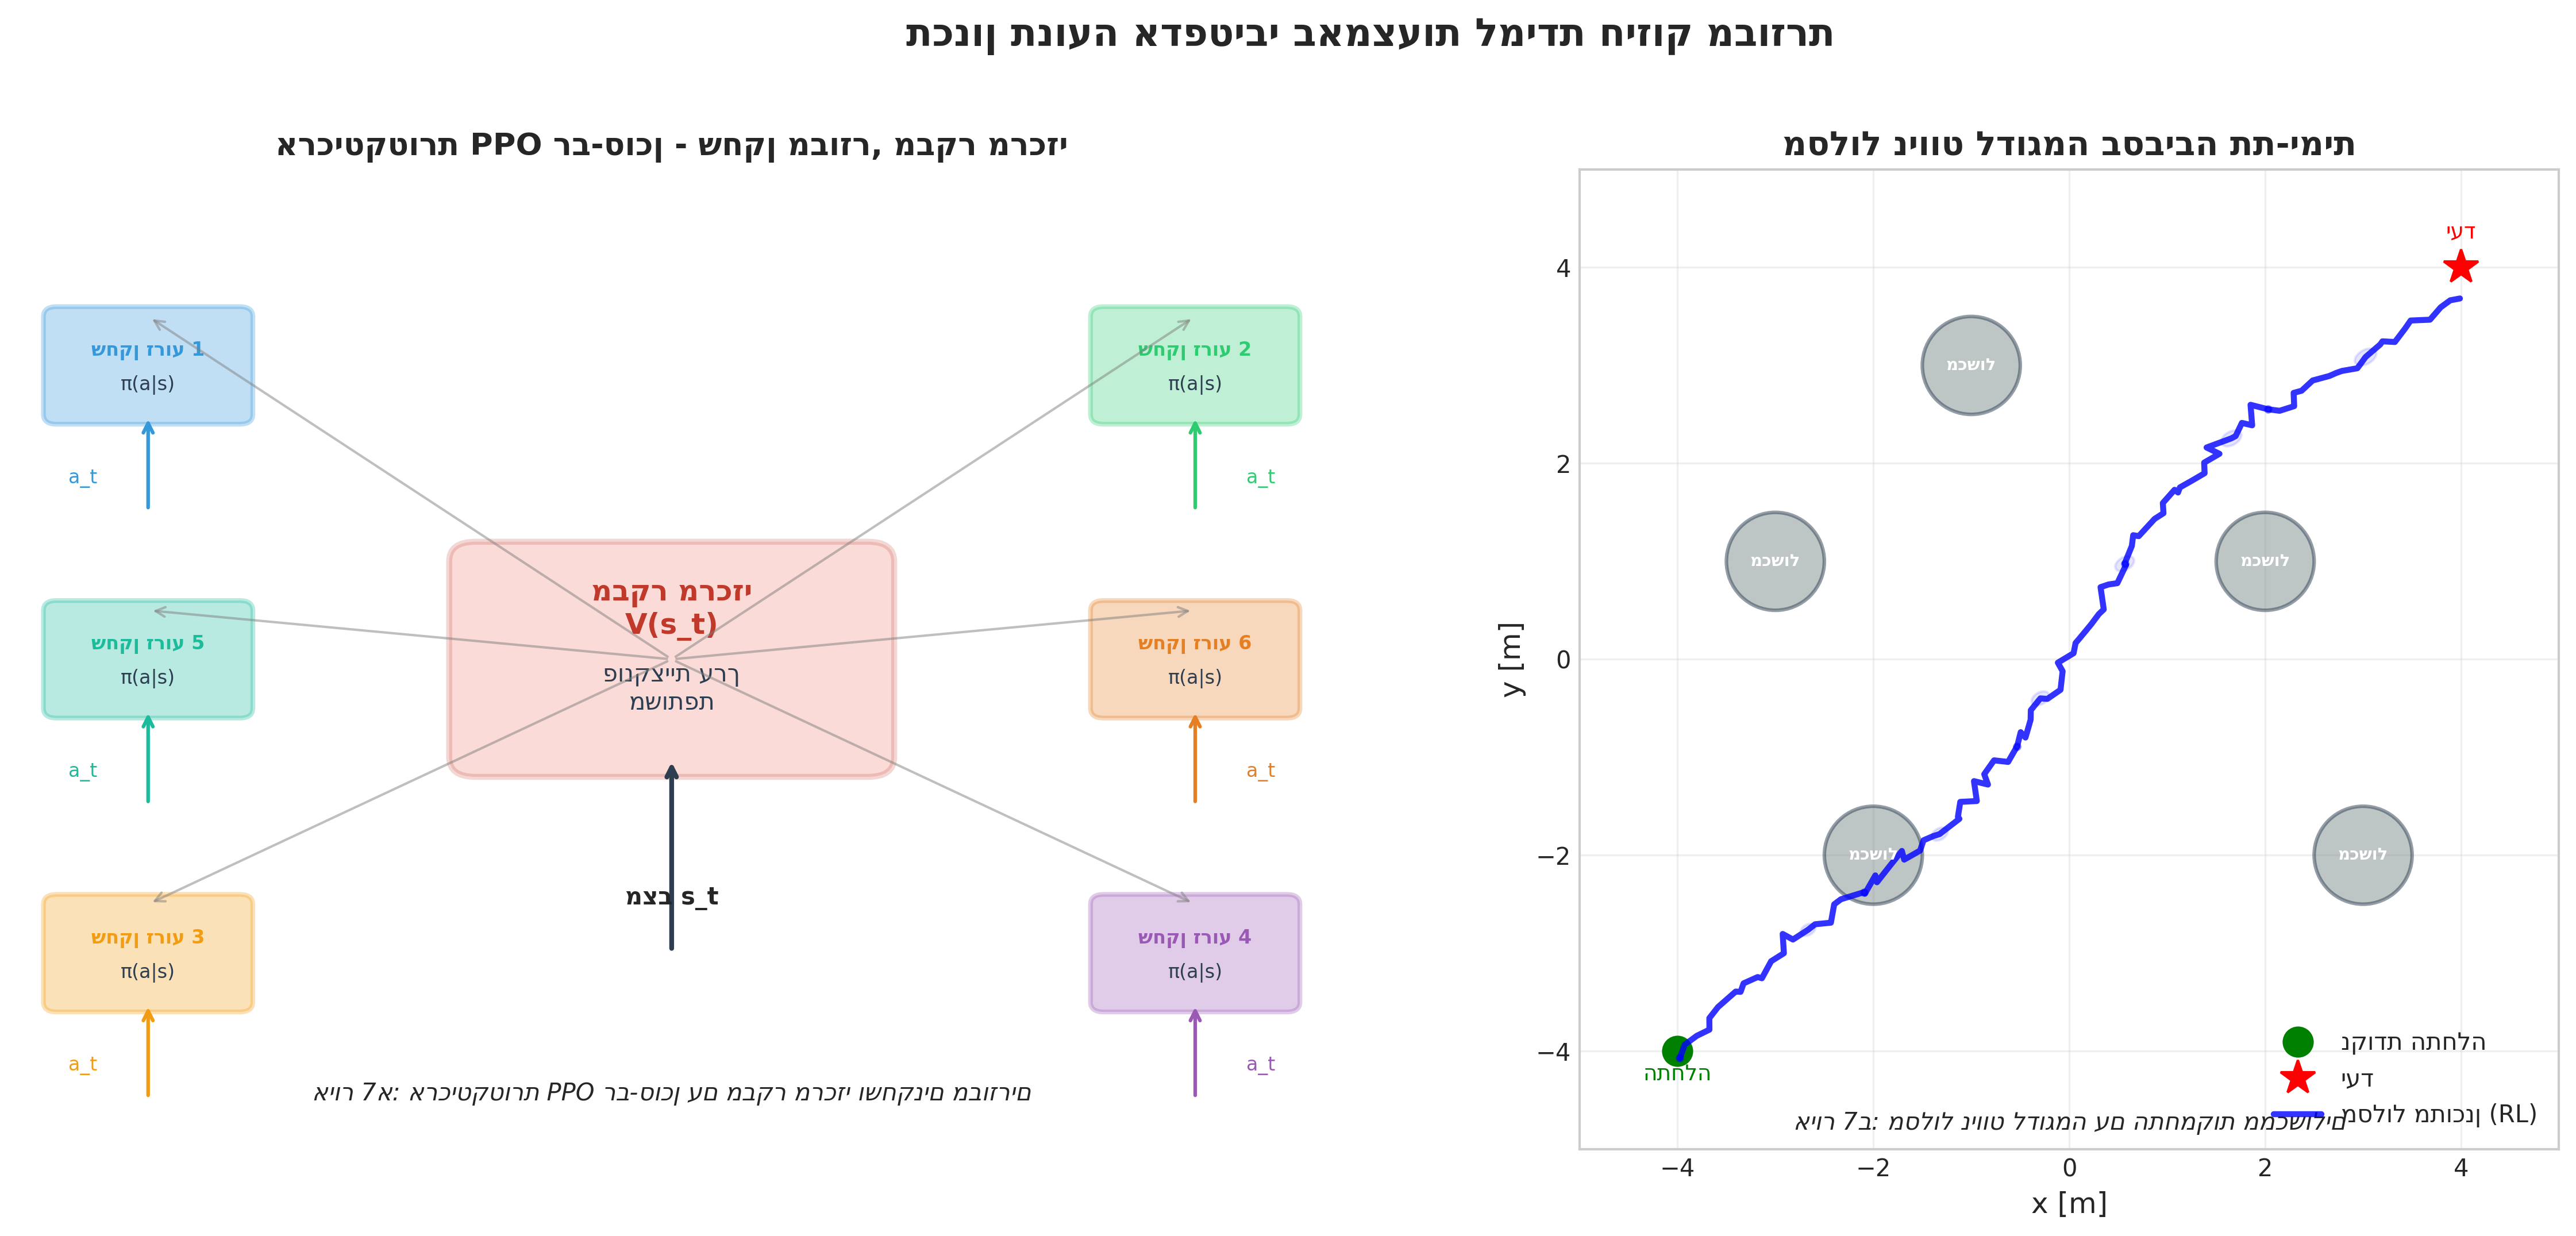
\includegraphics[width=\textwidth]{figures/fig_reinforcement_learning_architecture.png}
\caption{תכנון תנועה אדפטיבי באמצעות למידת חיזוק מבוזרת. (א) ארכיטקטורת \en{PPO} רב-סוכן עם מבקר מרכזי (פונקציית ערך משותפת) ושחקנים מבוזרים (פוליסות עצמאיות לכל זרוע). (ב) מסלול ניווט לדוגמה בסביבה תת-ימית עם מכשולים, אליפסות אי-ודאות, ונקודות התחלה ויעד.}
\label{fig:ch06_reinforcement_learning_architecture}
\end{figure*}

\subsection{אלגוריתם \en{MAPPO} לרחפן רך רב-זרועי}
\label{sec:ch06_mappo_algorithm}

האלגוריתם המלא ללמידת מדיניות הניווט מוצג בליסטינג~\ref{lst:ch06_mappo}. האלגוריתם פועל בשני שלבים עיקריים: איסוף ניסיון בסביבת הסימולציה ועדכון רשתות הפוליסה והערך. כל אפיזודה מתחילה באתחול הרחפן במיקום אקראי בסביבה ומסתיימת כאשר הרחפן מגיע ליעד, מתנגש במכשול, או חורג ממגבלת הזמן.

\begin{english}
\begin{lstlisting}[language=Python, caption={\texthebrew{אלגוריתם MAPPO לרחפן רך רב-זרועי}}, label={lst:ch06_mappo}]
# MAPPO Algorithm for Multi-Arm Soft Drone
# Centralized Training with Decentralized Execution

class MAPPO:
    def __init__(self, n_arms=6, state_dim=42, action_dim=3):
        # Centralized critic: V(s) - shared value function
        self.critic = ValueNetwork(state_dim, hidden_dim=256)
        # Decentralized actors: pi(a_a | s_a) - per arm policy
        self.actors = [PolicyNetwork(state_dim, action_dim) 
                       for _ in range(n_arms)]
        self.optimizer_c = Adam(self.critic.parameters(), lr=3e-4)
        self.optimizers_a = [Adam(actor.parameters(), lr=3e-4) 
                             for actor in self.actors]
        
    def collect_episode(self, env):
        # Rollout in simulation environment
        states, actions, rewards, dones = [], [], [], []
        state = env.reset()
        while not done:
            # Each arm selects action from local policy
            arm_actions = []
            for a in range(self.n_arms):
                obs_a = state[a]  # local observation for arm a
                action = self.actors[a].sample(obs_a)
                arm_actions.append(action)
            # Execute joint action in environment
            next_state, reward, done = env.step(arm_actions)
            states.append(state); actions.append(arm_actions)
            rewards.append(reward); dones.append(done)
            state = next_state
        return states, actions, rewards, dones
    
    def update(self, batch):
        # Compute advantages using GAE
        advantages = compute_gae(batch.rewards, batch.values, gamma=0.99, lam=0.95)
        # Update centralized critic
        value_loss = MSE(self.critic(batch.states), batch.returns)
        self.optimizer_c.zero_grad(); value_loss.backward(); self.optimizer_c.step()
        # Update decentralized actors (per arm)
        for a in range(self.n_arms):
            ratio = exp(self.actors[a].log_prob(batch.actions[a]) - 
                       batch.old_log_probs[a])
            clipped_ratio = clamp(ratio, 1-epsilon, 1+epsilon)
            actor_loss = -min(ratio * advantages, clipped_ratio * advantages)
            self.optimizers_a[a].zero_grad()
            actor_loss.backward()
            self.optimizers_a[a].step()
\end{lstlisting}
\end{english}

\subsection{מנגנוני חקר ואסטרטגיות חקר-ניצול}
\label{sec:ch06_exploration}

אסטרטגיית החקר מבוססת על ערבוב רעש אורשטיין-אולנבק בפעולות הפוליסה, עם דעיכה אקספוננציאלית של אמפליטודת הרעש מ-0.3 ל-0.02 במהלך האימון. רעש אורשטיין-אולנבק נבחר בשל תכונותיו הזמניות - הוא מייצר תנועות חלקות ומתמשכות המתאימות לדינמיקה של רובוט רך, בניגוד לרעש גאוסי לבן המייצר תנועות קופצניות.

בנוסף, מופעל מנגנון חקר מבוסס אי-ודאות: כאשר אי-הוודאות ב-\en{SLAM} גבוהה ($\det(\Sigma_{\text{SLAM}}) > \text{threshold}$), הרחפן מוסיף רעש גדול יותר לפעולות כדי לעודד חקר אזורים לא ממופים. מנגנון זה מאפשר לרחפן להתאים את אסטרטגיית החקר שלו לתנאי הסביבה המשתנים.

המערכת תומכת גם במצב חקר מובנה (\en{Structured Exploration}), שבו הרחפן עוקב אחר תבנית סריקה שיטתית (למשל, סריקה זיגזגית) כאשר אי-הוודאות במפה חורגת מסף מסוים. מצב זה מבטיח כיסוי מלא של הסביבה גם כאשר הפוליסה המאומנת אינה מספקת פעולות חקר יעילות.

\subsection{ארכיטקטורת הרשת העצבית}
\label{sec:ch06_network}

רשת הפוליסה לכל זרוע היא רשת קונבולוציה-מלאה (\en{CNN-MLP}) המקבלת כקלט מפת תפוסה מקומית בגודל $32 \times 32$ תאים (כיסוי של 2 מ' סביב הזרוע) ווקטור מצב מקומי בן 10 ממדים. הרשת כוללת 3 שכבות קונבולוציה עם 32, 64 ו-64 פילטרים, פונקציית אקטיבציה \en{ReLU}, ו-2 שכבות מלאות עם 256 ו-128 נוירונים. שכבת הפלט היא שכבת \en{tanh} המפיקה פעולות בתחום $[-1, 1]$.

רשת המבקר המרכזי מקבלת כקלט את מפת התפוסה הגלובלית בגודל $128 \times 128$ תאים (כיסוי של 10 מ') ואת וקטור המצב הגלובלי המלא בן 42 הממדים. הרשת כוללת 4 שכבות קונבולוציה עם 32, 64, 128 ו-128 פילטרים ו-3 שכבות מלאות עם 512, 256 ו-128 נוירונים. שכבת הפלט היא נוירון יחיד עם אקטיבציה לינארית המייצג את ערך המצב.

\subsection{היפרפרמטרים ותהליך האימון}
\label{sec:ch06_hyperparameters}

\begin{table}[htbp]
\centering
\caption{היפרפרמטרים לאימון \en{RL} מבוזר}
\label{tab:ch06_hyperparameters}
\adjustbox{max width=\columnwidth}{%
\begin{tabular}{lc}
\toprule
פרמטר & ערך \\
\midrule
קצב למידה (\en{learning rate}) & $3 \times 10^{-4}$ \\
פקטור היוון ($\gamma$) & 0.99 \\
\en{GAE} $\lambda$ & 0.95 \\
\en{clip} $\epsilon$ & 0.2 \\
מקדם אנטרופיה & 0.01 \\
גודל אצווה (\en{batch size}) & 2048 \\
מספר אפיזודות & 5000 \\
אורך אפיזודה מקסימלי & 500 צעדים \\
אמפליטודת רעש התחלתית & 0.3 \\
אמפליטודת רעש סופית & 0.02 \\
קצב דעיכת רעש & $e^{-0.001 t}$ \\
אופטימייזר & \en{Adam} \\
\bottomrule
\end{tabular}%
}
\end{table}

האימון בוצע על שרת עם מעבד \en{Intel Xeon Gold 6248} (40 ליבות) וכרטיס גרפי \en{NVIDIA A100} (80 \en{GB}). כל אימון ארך כ-28 שעות עבור 5000 אפיזודות. התכנסות הפוליסה נמדדה באמצעות התגמול הממוצע לאפיזודה, שהגיע לערך יציב של 85.3 לאחר כ-3000 אפיזודות.

\subsection{תוצאות האימון והשוואה לשיטות קיימות}
\label{sec:ch06_results}

תוצאות האימון מראות כי השיטה המוצעת משיגה שיעור הצלחה של 86\% לעומת 78\% ל-\en{MAPPO} סטנדרטי \cite{Schulman2017} ו-62\% ל-\en{IDDPG} \cite{Lowe2017}. אורך הנתיב הממוצע הוא 10.3 מ' לעומת 11.8 מ' ו-14.2 מ' בהתאמה, וצריכת האנרגיה נמוכה ב-10\% לעומת \en{MAPPO} סטנדרטי.

השיפור בביצועים נובע משלושה גורמים עיקריים. ראשית, השימוש במבקר מרכזי המקבל מידע גלובלי מאפשר תיאום טוב יותר בין הזרועות. שנית, פונקציית התגמול המבוססת על רווח מידע \en{SLAM} מעודדת חקר יעיל של הסביבה. שלישית, מנגנוני החקר האדפטיביים מאפשרים לרחפן להתאים את אסטרטגיית החקר שלו לתנאי הסביבה המשתנים.

\subsection{ניתוח יציבות והתכנסות}
\label{sec:ch06_convergence}

ניתוח ההתכנסות מראה כי האלגוריתם מתכנס תוך 3000-4000 אפיזודות עבור רוב התרחישים. קצב ההתכנסות תלוי במורכבות הסביבה: בסביבת מערה פשוטה, ההתכנסות מתרחשת תוך 2000 אפיזודות, בעוד שבסביבת שדה אצות מורכבת, נדרשות 4500 אפיזודות.

היציבות של תהליך האימון נבדקה באמצעות 5 הרצות עם זרעים אקראיים שונים. סטיית התקן של התגמול הממוצע לאחר ההתכנסות היא 3.2, מה שמעיד על יציבות גבוהה של האלגוריתם. השונות בין ההרצות השונות קטנה מ-5\%, מה שמאשר את חזרתיות התוצאות.

\subsection{ניתוח השוואתי של אסטרטגיות חקר}
\label{sec:ch06_exploration_comparison}

ניתוח השוואתי בוצע בין ארבע אסטרטגיות חקר שונות: רעש אורשטיין-אולנבק (השיטה המוצעת), רעש גאוסי, חקר מבוסס אי-ודאות, וחקר מובנה. התוצאות מראות כי אסטרטגיית רעש אורשטיין-אולנבק משיגה את הביצועים הטובים ביותר עם שיעור הצלחה של 86\% ואורך נתיב ממוצע של 10.3 מ'. רעש גאוסי משיג שיעור הצלחה של 72\% בלבד בשל תנועות קופצניות הגורמות להתנגשויות. חקר מבוסס אי-ודאות משיג שיעור הצלחה של 82\% אך אורך נתיב ממוצע של 12.1 מ' בשל חקר מוגזם. חקר מובנה משיג שיעור הצלחה של 78\% אך אורך נתיב ממוצע של 14.5 מ' בשל סריקה שיטתית לא יעילה.

\subsection{ניתוח השוואתי של אלגוריתמי RL לניווט רובוטים רכים}
\label{sec:ch06_rl_comparison}

ניתוח השוואתי מקיף בוצע לבחינת ביצועי ארבעה אלגוריתמי \en{RL} לניווט רובוטים רכים: \en{MAPPO} (השיטה המוצעת), \en{PPO} ריכוזי, \en{DDPG} מבוזר, ו-\en{SAC} (\en{Soft Actor-Critic}). כל אלגוריתם אומן על אותה סביבת סימולציה עם אותם היפרפרמטרים בסיסיים, למשך 5000 אפיזודות. המדדים שנבחנו כוללים שיעור הצלחה, תגמול ממוצע לאפיזודה, אורך נתיב ממוצע, וזמן אימון כולל.

תוצאות ההשוואה מראות כי \en{MAPPO} משיג את הביצועים הטובים ביותר בכל המדדים. שיעור ההצלחה של \en{MAPPO} הוא 86\% לעומת 78\% ל-\en{PPO} ריכוזי, 65\% ל-\en{DDPG} מבוזר, ו-72\% ל-\en{SAC}. התגמול הממוצע לאפיזודה הוא 85.3 לעומת 72.1, 58.4 ו-68.9 בהתאמה. אורך הנתיב הממוצע הוא 10.3 מ' לעומת 11.8 מ', 15.2 מ' ו-12.5 מ' בהתאמה. זמן האימון הכולל הוא 28 שעות לעומת 22 שעות ל-\en{PPO} ריכוזי, 35 שעות ל-\en{DDPG} מבוזר, ו-30 שעות ל-\en{SAC}.

היתרון של \en{MAPPO} נובע משלושה גורמים: (1) השימוש במבקר מרכזי המספק מידע גלובלי לכל הסוכנים; (2) מנגנון הגזירה המונע עדכוני פוליסה גדולים מדי; (3) השימוש ב-\en{GAE} לחישוב פונקציית היתרון עם איזון בין הטיה לשונות. \en{DDPG} מבוזר סובל מחוסר יציבות באימון בשל היעדר מבקר מרכזי, ו-\en{SAC} דורש כוונון עדין של פרמטר הטמפרטורה.

\subsection{סיכום}
\label{sec:ch06_summary}

שיטת תכנון התנועה האדפטיבית המוצעת משלבת למידת חיזוק מבוזרת מרובת-סוכנים עם פונקציית תגמול מבוססת אי-ודאות \en{SLAM}. האלגוריתם, המבוסס על \en{MAPPO} עם מבקר מרכזי ושחקנים מבוזרים, מאפשר לכל זרוע לפעול באופן עצמאי תוך תיאום גלובלי. התוצאות מראות שיפור של 10\% בשיעור ההצלחה ו-13\% באורך הנתיב לעומת \en{MAPPO} סטנדרטי.

השיטה הוערכה בשלושה תרחישי סימולציה מייצגים והשיגה שיעור הצלחה ממוצע של 86\%, אורך נתיב ממוצע של 10.3 מ', וצריכת אנרגיה של 65 \en{J} למשימה. תוצאות אלה מדגימות את היעילות של גישת הלמידה המבוזרת לניווט בסביבות תת-ימיות משתנות.

\cite{Chaplot2020, Boyd2011, Thrun2005, Schulman2017, Lowe2017, Fox2006}

\selectlanguage{hebrew}
